\section{Theorie}

\begin{align}
    \intertext{Unter Ultraschall werden Longitudinalwellen die eine Frequenz von ca. $20\, \unit{\kilo\hertz}$ bis $1\,\unit{\giga\hertz}$ verstanden. 
    Diese sind nicht in dem hörbaren Frequenzbereich der Menschen, welcher sich auf $ 16\,\unit{\hertz} $ bis $ 29\,\unit{\kilo\hertz} $ begrenzt.
    Einer von zwei Effekten ist der Doppler-Effekt.
    Bei diesem Effekt bewegen sich Beobachter und Schallquelle relativ zueinander und die Änderung der dabei auftretenden Frequenz ist der sogenannte Doppler-Effekt.
    Die Richtung, in welche sich die Schallquelle bewegt, spielt dabei eine wichtige Rolle.
    Bewegt sich die Schallquelle von dem Beobachter weg, wird die Frequenz zu einer kleineren verschoben $\nu_{\text{gr}}$.
    Bewegt sich die Schallquelle hingegen auf den Beobachter zu, wird die Frequenz zu einer höheren verschoben $\nu_{\text{kl}}$.}
    \nu_\text{{kl/gr}} = \frac{\nu_{0}}{1 \pm \frac{v}{c}} \label{1}
    \intertext{Das $\nu_{0}$ steht dabei für die Ausgangsfrequenz.
    Wenn sich der Beobachter bewegt und die Quelle ruht sieht dies jedoch anders aus.
    Bewegt sich der Beobachter auf die Quelle zu, wird die Frequenz zu einer höheren verschoben $\nu_{\text{h}}$.
    Bewegt sich der Beobachter von der Quelle weg, wir die Frequenz zu einer niedrigeren verschoben $\nu_{\text{n}}$.}
    \nu_\text{{h/n}} = \nu_{0}\,\left( 1 \pm \frac{v}{c}\right). \label{2}
    \intertext{Verwendung findet dieser Effekt Beispielsweise in der Medizin um Blutströmungsgeschwindigkeiten zu bestimmen. 
    Dabei trifft die Ultraschallwelle auf das Blutkörperchen und durch den Doppler-Effekt wird die Frequenz verschoben um}
    \increment \nu = \nu_{0}\frac{v}{c}\left(\cos\alpha + \cos\beta\right) \label{3}
    \intertext{ Hierbei ist v die Geschwindigkeit des Blutes, c die Schallgeschwindigkeit und $\alpha$ und $\beta$ die Winkel, in welchen die Ultraschallwellen auf die Blutkörperchen auftreffen.
    Die Winkel \alpha und \beta sind bei diesem Verfahren, Impuls-Echo-Verfahren, identisch. 
    Dadurch folgt die Frequenzverschiebung durch}
    \increment \nu = 2\nu_{0}\frac{v}{c} \cos \alpha \label{4}
\end{align}

\begin{figure}[H]       
    \centering
    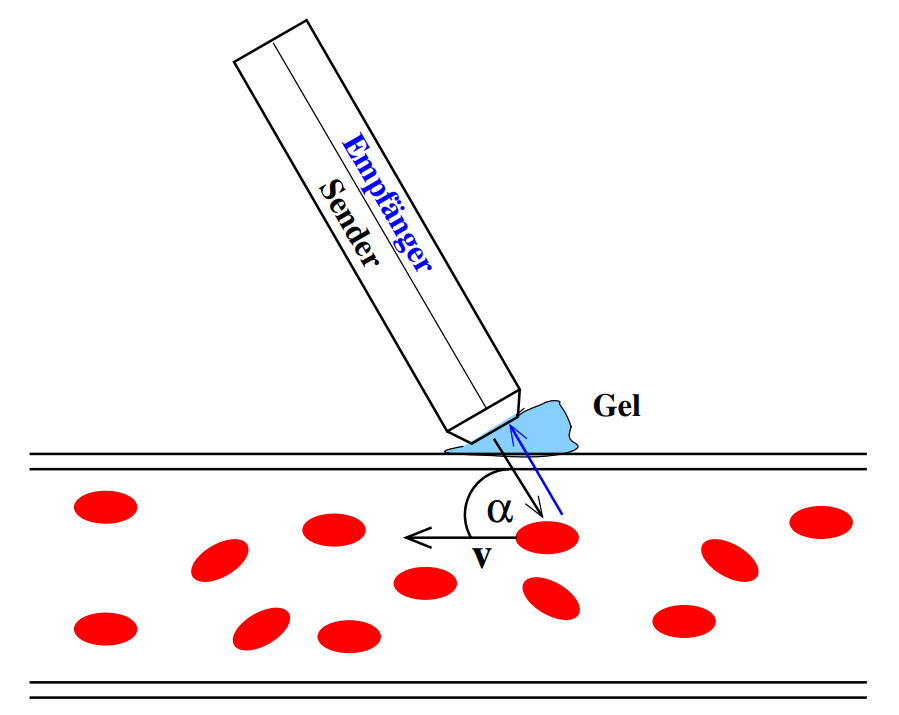
\includegraphics[height=60mm]{bilder/Frequenzverschiebung.png}
    \caption{Verbildlichung der Frequenzverschiebung durch den Doppler Effekt \cite{a1}.\label{Abbildung1} }
\end{figure}

\begin{flushleft}
    Eine von vielen Methoden Ultraschallwellen zu erzeugen ist die Anwendung von dem reziproken piezo-elektrischen Effekt.
    Hierbei wird ein piezoelektrischer Kristall in Schwingung gebracht, indem der Kristall in ein elektrisches Wechselfeld gebracht wird.
    Beim Schwingen werden Ultraschallwellen abgestrahlt und bei Übereinstimmung der Eigenfrequenz des Kristalls mit der Frequenz des Anregers, so können wiederum große Schwingamplituden erzeugt werden mit sehr hohen Energiedichten.
\end{flushleft}

\begin{flushleft}
    Der Piezokristall kann nicht nur als Schallsender sondern auch als Schallempfänger verwendet werden, wobei Schallwellen auf den Kristall treffen und diesen zum Schwingen bringen.
    Die Ultraschallsonde die in diesem Versuch verwendet wird ist Ultraschallsender sowie Empfänger. 
\end{flushleft}